\documentclass{article}
\usepackage[pdftex]{hyperref}
\usepackage[pdftex]{graphicx}
\usepackage{fullpage}
\usepackage{color}
\usepackage{hyperref}
\usepackage{wrapfig}
\title{ORC File Format Specification}
\author{Owen O'Malley}
\date{October 2014}
\begin{document}
\maketitle

\section{Introduction}

\begin{wrapfigure}{r}{3.1in}
  \centering
  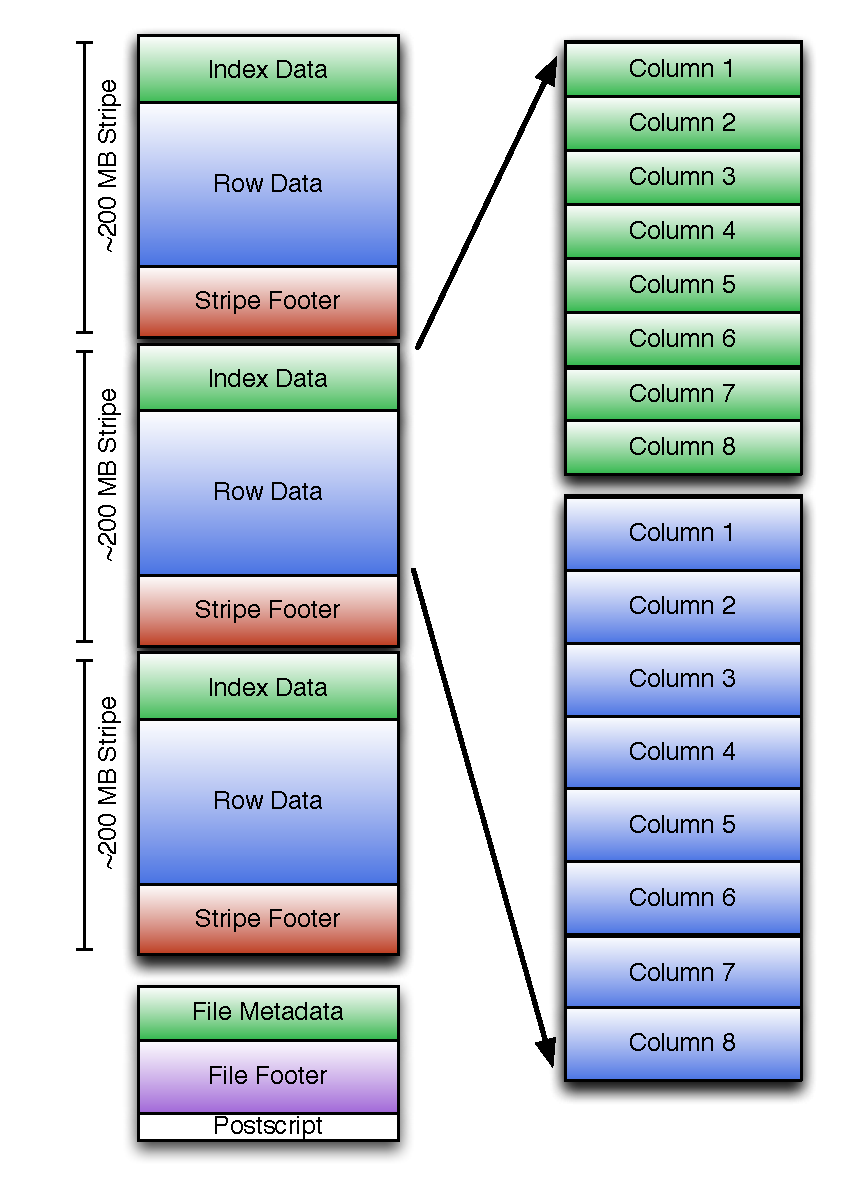
\includegraphics[width=3in]{ORCFileStructure.pdf}
  \caption{ORC file top level structure}
  \label{orc-structure}
  \vspace{-20pt}
\end{wrapfigure}

Hive's RCFile was the standard format for storing tabular data in
Hadoop for several years. However, RCFile has limitations because it
treats each column as a binary blob without semantics. In Hive 0.11 we
added a new file format named Optimized Row Columnar (ORC) file that
uses and retains the type information from the table definition. ORC
uses type specific readers and writers that provide light weight
compression techniques such as dictionary encoding, bit packing, delta
encoding, and run length encoding -- resulting in dramatically smaller
files. Additionally, ORC can apply generic compression using zlib, or
Snappy on top of the lightweight compression for even smaller
files. However, storage savings are only part of the gain. ORC
supports projection, which selects subsets of the columns for reading,
so that queries reading only one column read only the required
bytes. Furthermore, ORC files include light weight indexes that
include the minimum and maximum values for each column in each set of
10,000 rows and the entire file. Using pushdown filters from Hive, the
file reader can skip entire sets of rows that aren't important for
this query.

\section{File Tail}

Since HDFS does not support changing the data in a file after it is
written, ORC stores the top level index at the end of the file. The
overall structure of the file is given in figure~\ref{orc-structure}.
The file's tail consists of 3 parts- the file metadata, file footer,
and postscript. 

The metadata for ORC is stored using
\href{http://s.apache.org/protobuf_encoding}{Protocol Buffers}, which
provides the ability to add new fields without breaking readers. This
document incorporates the Protobuf definition from the
\href{http://s.apache.org/orc_proto}{ORC source code} and the reader
is encouraged to review the Protobuf encoding if they need to understand
the byte-level encoding

\subsection{Postscript}

The Postscript section provides the necessary information to interpret
the rest of the file including the length of the file's Footer and
Metadata sections, the version of the file, and the kind of general
compression used (eg. none, zlib, or snappy). The Postscript is never
compressed and ends one byte before the end of the file.  The version
stored in the Postscript is the lowest version of Hive that is
guaranteed to be able to read the file and it stored as a sequence of
the major and minor version. There are currently two versions that are
used: [0,11] for Hive 0.11, and [0,12] for Hive 0.12 to 0.14.

The process of reading an ORC file works backwards through the
file. Rather than making multiple short reads, the ORC reader reads
the last 16k bytes of the file with the hope that it will contain both
the Footer and Postscript sections. The final byte of the file
contains the serialized length of the Postscript, which must be less
than 256 bytes. Once the Postscript is parsed, the compressed
serialized length of the Footer is known and it can be decompressed
and parsed.

\begin{verbatim}
message PostScript {
  // the length of the footer section in bytes
  optional uint64 footerLength = 1;
  // the kind of generic compression used
  optional CompressionKind compression = 2;
  // the maximum size of each compression chunk
  optional uint64 compressionBlockSize = 3;
  // the version of the writer
  repeated uint32 version = 4 [packed = true];
  // the length of the metadata section in bytes
  optional uint64 metadataLength = 5;
  // the fixed string "ORC"
  optional string magic = 8000;
}

enum CompressionKind {
  NONE = 0;
  ZLIB = 1;
  SNAPPY = 2;
  LZO = 3;
}
\end{verbatim}

\subsection{Footer}

The Footer section contains the layout of the body of the file, the
type schema information, the number of rows, and the statistics about
each of the columns. 

The file is broken in to three parts- Header, Body, and Tail. The
Header consists of the bytes ``ORC'' to support tools that want to
scan the front of the file to determine the type of the file. The Body
contains the rows and indexes, and the Tail gives the file level
information as described in this section.

\begin{verbatim}
message Footer {
  // the length of the file header in bytes (always 3)
  optional uint64 headerLength = 1;
  // the length of the file body in bytes
  optional uint64 contentLength = 2;
  // the information about the stripes
  repeated StripeInformation stripes = 3;
  // the schema information
  repeated Type types = 4;
  // the user metadata that was added
  repeated UserMetadataItem metadata = 5;
  // the total number of rows in the file
  optional uint64 numberOfRows = 6;
  // the statistics of each column across the file
  repeated ColumnStatistics statistics = 7;
  // the maximum number of rows in each index entry
  optional uint32 rowIndexStride = 8;
}
\end{verbatim}

\subsubsection{Stripe Information}

The body of the file is divided into stripes. Each stripe is self
contained and may be read using only its own bytes combined with the
file's Footer and Postscript. Each stripe contains only entire rows so
that rows never straddle stripe boundaries. Stripes have three
sections: a set of indexes for the rows within the stripe, the data
itself, and a stripe footer. Both the indexes and the data sections
are divided by columns so that only the data for the required columns
needs to be read.

\begin{verbatim}
message StripeInformation {
  // the start of the stripe within the file
  optional uint64 offset = 1;
  // the length of the indexes in bytes
  optional uint64 indexLength = 2;
  // the length of the data in bytes
  optional uint64 dataLength = 3;
  // the length of the footer in bytes
  optional uint64 footerLength = 4;
  // the number of rows in the stripe
  optional uint64 numberOfRows = 5;
}
\end{verbatim}

\subsubsection{Type Information}

\begin{wrapfigure}{r}{2.5in}
  \centering
  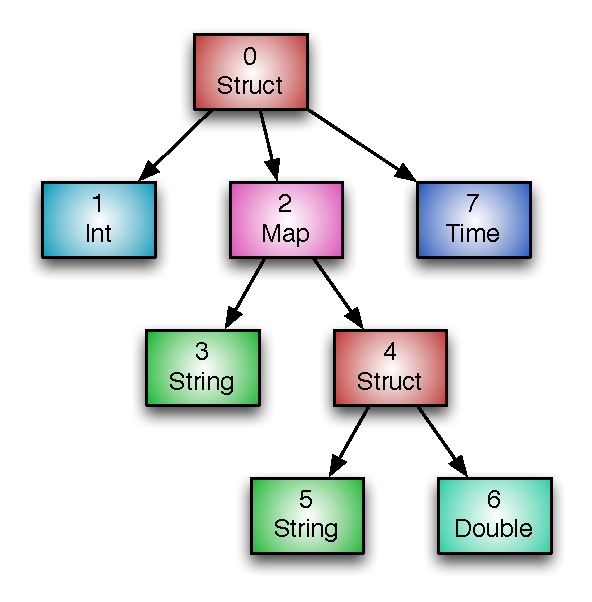
\includegraphics[width=2.4in]{TreeWriters.pdf}
  \caption{Type Tree}
  \label{type-tree}
  \vspace{-100pt}
\end{wrapfigure}

All of the rows in an ORC file must have the same schema.  Logically
the schema is expressed as a tree as in figure~\ref{type-tree}, where
the compound types have subcolumns under them. 

The equivalent Hive DDL for figure~\ref{type-tree} would be:
\begin{verbatim}
create table Foobar (
  myInt int,
  myMap map<string, 
            struct<myString : string, 
                   myDouble: double>>,
  myTime timestamp
);
\end{verbatim}

The type tree is flattened in to a list via a pre-order traversal
where each type is assigned the next id. Clearly the root of the type
tree is always type id 0. Compound types have a field named subtypes
that contains the list of their children's type ids.

\begin{verbatim}
message Type {
  enum Kind {
    BOOLEAN = 0;
    BYTE = 1;
    SHORT = 2;
    INT = 3;
    LONG = 4;
    FLOAT = 5;
    DOUBLE = 6;
    STRING = 7;
    BINARY = 8;
    TIMESTAMP = 9;
    LIST = 10;
    MAP = 11;
    STRUCT = 12;
    UNION = 13;
    DECIMAL = 14;
    DATE = 15;
    VARCHAR = 16;
    CHAR = 17;
  }
  // the kind of this type
  required Kind kind = 1;
  // the type ids of any subcolumns for list, map, struct, or union
  repeated uint32 subtypes = 2 [packed=true];
  // the list of field names for struct
  repeated string fieldNames = 3;
  // the maximum length of the type for varchar or char
  optional uint32 maximumLength = 4;
  // the precision and scale for decimal
  optional uint32 precision = 5;
  optional uint32 scale = 6;
}
\end{verbatim}

\subsubsection{Column Statistics}

The goal of the column statistics is that for each column, the writer
records the count and depending on the type other useful fields.  For
most of the primitive types, it records the minimum and maximum
values; and for numeric types it additionally stores the sum.

\begin{verbatim}
message ColumnStatistics {
  // the number of values
  optional uint64 numberOfValues = 1;

  // At most one of these has a value for any column
  optional IntegerStatistics intStatistics = 2;
  optional DoubleStatistics doubleStatistics = 3;
  optional StringStatistics stringStatistics = 4;
  optional BucketStatistics bucketStatistics = 5;
  optional DecimalStatistics decimalStatistics = 6;
  optional DateStatistics dateStatistics = 7;
  optional BinaryStatistics binaryStatistics = 8;
  optional TimestampStatistics timestampStatistics = 9;
}
\end{verbatim}

For integer types (tinyint, smallint, int, bigint), the column
statistics includes the minimum, maximum, and sum. If the sum
overflows long at any point during the calculation, no sum is
recorded.

\begin{verbatim}
message IntegerStatistics  {
  optional sint64 minimum = 1;
  optional sint64 maximum = 2;
  optional sint64 sum = 3;
}
\end{verbatim}

For floating point types (float, double), the column statistics
include the minimum, maximum, and sum. If the sum overflows a double,
no sum is recorded.

\begin{verbatim}
message DoubleStatistics {
  optional double minimum = 1;
  optional double maximum = 2;
  optional double sum = 3;
}
\end{verbatim}

For strings, the minimum value, maximum value, and the sum of the
lengths of the values are recorded.

\begin{verbatim}
message StringStatistics {
  optional string minimum = 1;
  optional string maximum = 2;
  // sum will store the total length of all strings
  optional sint64 sum = 3;
}
\end{verbatim}

For booleans, the statistics include the count of false and true values.

\begin{verbatim}
message BucketStatistics {
  repeated uint64 count = 1 [packed=true];
}
\end{verbatim}

For decimals, the minimum, maximum, and sum are stored.

\begin{verbatim}
message DecimalStatistics {
  optional string minimum = 1;
  optional string maximum = 2;
  optional string sum = 3;
}
\end{verbatim}

Date columns record the minimum and maximum values as the number of days since
the epoch (1/1/2015).

\begin{verbatim}
message DateStatistics {
  // min,max values saved as days since epoch
  optional sint32 minimum = 1;
  optional sint32 maximum = 2;
}
\end{verbatim}

Timestamp columns record the minimum and maximum values as the number of 
milliseconds since the epoch (1/1/2015).

\begin{verbatim}
message TimestampStatistics {
  // min,max values saved as milliseconds since epoch
  optional sint64 minimum = 1;
  optional sint64 maximum = 2;
}
\end{verbatim}

Binary columns store the aggregate number of bytes across all of the values.

\begin{verbatim}
message BinaryStatistics {
  // sum will store the total binary blob length
  optional sint64 sum = 1;
}
\end{verbatim}

\subsubsection{User Metadata}

The user can add arbitrary key/value pairs to an ORC file as it is
written. The contents of the keys and values are completely
application defined, but the key is a string and the value is
binary. Care should be taken by applications to make sure that their
keys are unique and in general should be prefixed with an organization
code.

\begin{verbatim}
message UserMetadataItem {
  // the user defined key
  required string name = 1;
  // the user defined binary value
  required bytes value = 2;
}
\end{verbatim}

\subsection{File Metadata}

The file Metadata section contains column statistics at the stripe
level granularity. These statistics enable input split elimination
based on the predicate push-down evaluated per a stripe.

\begin{verbatim}
message StripeStatistics {
  repeated ColumnStatistics colStats = 1;
}

message Metadata {
  repeated StripeStatistics stripeStats = 1;
}
\end{verbatim}

\section{Compression Streams}

\begin{wrapfigure}{r}{2.5in}
  \centering
  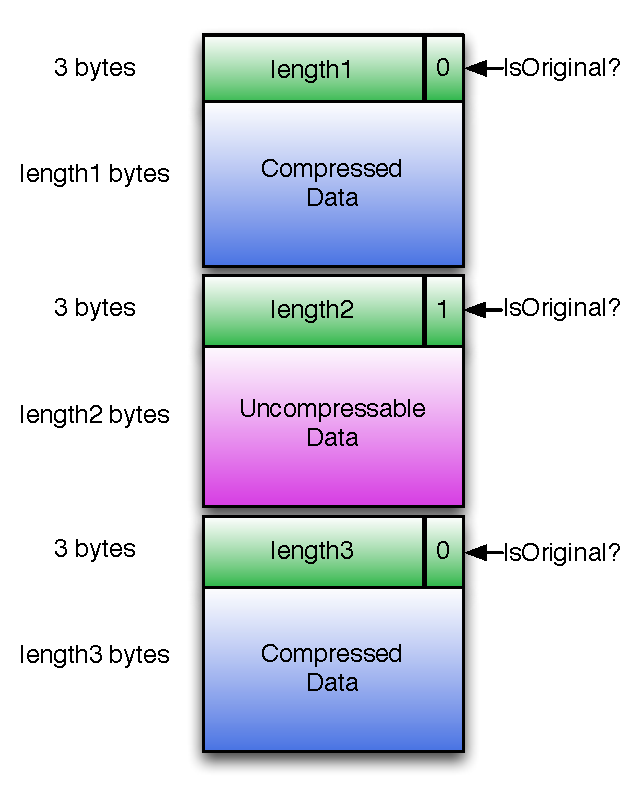
\includegraphics[width=2.4in]{CompressionStream.pdf}
  \caption{Compression Stream Structure}
  \label{compression-stream}
  \vspace{-40pt}
\end{wrapfigure}

If the ORC file writer selects a generic compression codec (zlib or
snappy), every part of the ORC file except for the Postscript is
compressed with that codec.  However, one of the requirements for ORC
is that the reader be able to skip over compressed bytes without
decompressing the entire stream. To manage this, ORC writes compressed
streams in chunks with headers as in figure~\ref{compression-stream}.
To handle uncompressable data, if the compressed data is larger than
the original, the original is stored and the isOriginal flag is
set. Each header is 3 bytes long with $ compressedLength * 2 +
isOriginal $ stored as a little endian value. For example, the header
for a chunk that compressed to 100,000 bytes would be [0x40, 0x0d,
0x03]. The header for 5 bytes that did not compress would be [0x0b,
0x00, 0x00]. Each compression chunk is compressed independently so
that as long as a decompressor starts at the top of a header, it can
start decompressing without the previous bytes.

The default compression chunk size is 256K, but writers can choose
their own value less than $2^{23}$.  Larger chunks lead to better
compression, but require more memory.  The chunk size is recorded in
the Postscript so that readers can allocate appropriately sized
buffers.

ORC files without generic compression write each stream directly
with no headers.

\section{Run Length Encoding}

\subsection{Base 128 Varint}

Variable width integer encodings take advantage of the fact that most
numbers are small and that having smaller encodings for small numbers
shrinks the overall size of the data. ORC uses the varint format from
Protocol Buffers, which writes data in little endian format using the
low 7 bits of each byte. The high bit in each byte is set if the
number continues into the next byte.

\vspace{10pt}
\begin{tabular}{| c | c |}
\hline
Unsigned Orignal & Serialized \\
\hline
0 & 0x00 \\
1 & 0x01 \\
127 & 0x7f \\
128 & 0x80, 0x01 \\
129 & 0x81, 0x01 \\
16383 & 0xff, 0x7f \\
16384 & 0x80, 0x80, 0x01 \\
16385 & 0x81, 0x80, 0x01 \\
\hline
\end{tabular}
\vspace{10pt}

For signed integer types, the number is converted into an unsigned
number using a zigzag encoding.  Zigzag encoding moves the sign bit to
the least significant bit using the expression $(val << 1) \wedge (val
>> 63)$ and derives its name from the fact that positive and negative
numbers alternate once encoded. The unsigned number is then serialized
as above.

\vspace{10pt}
\begin{tabular}{| c | c |}
\hline
Signed Original & Unsigned\\
\hline
0 & 0 \\
-1 & 1 \\
1 & 2 \\
-2 & 3 \\
2 & 4 \\
\hline
\end{tabular}

\subsection{Byte Run Length Encoding}
\label{byte-rle}

For byte streams, ORC uses a very light weight encoding of identical
values.

\begin{description}
\item[Run] a sequence of at least 3 identical values
\item[Literals] a sequence of non-identical values
\end{description}

The first byte of each group of values is a header than determines
whether it is a run (value between 0 to 127) or literal list (value
between -128 to -1). For runs, the control byte is the length of the
run minus the length of the minimal run (3) and the control byte for
literal lists is the negative length of the list. For example, a
hundred 0's is encoded as [0x61, 0x00] and the sequence 0x44, 0x45
would be encoded as [0xfe, 0x44, 0x45]. The next group can choose
either of the encodings.

\subsection{Boolean Run Length Encoding}

For encoding boolean types, the bits are put in the bytes from most
significant to least significant. The bytes are encoded using byte run
length encoding as described in section~\ref{byte-rle}. For example,
the byte sequence [0xff, 0x80] would be one \verb+true+ followed by
seven \verb+false+ values.

\subsection{Integer Run Length Encoding version 1}

In Hive 0.11 ORC files used Run Length Enconding version 1 (RLEv1),
which provides a lightweight compression of signed or unsigned integer
sequences. RLEv1 has two sub-encodings:

\begin{description}
\item[Run] a sequence of values that differ by a small fixed delta
\item[Literals] a sequence of varint encoded values
\end{description}

Runs start with an initial byte of 0x00 to 0xf7, which encodes the
length of the run - 3. A second byte provides the fixed delta in the
range of -128 to 127. Finally, the first value of the run is encoded
as a base 128 varint.

For example, if the sequence is 100 instances of 7 the encoding would
start with $100 - 3$, followed by a delta of 0, and a varint of 7 for
an encoding of [0x61, 0x00, 0x07]. To encode the sequence of numbers
running from 100 to 1, the first byte is $100 - 3$, the delta is -1,
and the varint is 100 for an encoding of [0x61, 0xff, 0x64].

Literals start with an initial byte of 0x80 to 0xff, which corresponds
to the negative of number of literals in the sequence. Following the
header byte, the list of N varints is encoded.  Thus, if there are
no runs, the overhead is 1 byte for each 128 integers. The first 5
prime numbers [2, 3, 4, 7, 11] would encoded as [0xfb, 0x02, 0x03,
0x04, 0x07, 0xb].

\subsection{Integer Run Length Encoding Version 2}

In Hive 0.12, ORC introduced Run Length Encoding version 2 (RLEv2),
which has improved compression and fixed bit width encodings for
faster expansion. RLEv2 uses four sub-encodings based on the data:

\begin{description}
\item[Short Repeat] used for short sequences with repeated values
\item[Direct] used for random sequences with a fixed bit width
\item[Patched Base] used for random sequences with a variable bit width
\item[Delta] used for monotonically increasing or decreasing sequences
\end{description}

\subsubsection{Short Repeat}

The short repeat encoding is used for short repeating integer
sequences with the goal of minimizing the overhead of the header. All
of the bits listed in the header are from the first byte to the last
and from most significant bit to least significant bit. If the type is
signed, the value is zigzag encoded.

\begin{itemize}
\item 1 byte header
  \begin{itemize}
  \item 2 bits for encoding type (0)
  \item 3 bits for width (W) of repeating value (1 to 8 bytes)
  \item 3 bits for repeat count (3 to 10 values)
  \end{itemize}
\item W bytes in big endian format, which is zigzag encoded if they type
  is signed
\end{itemize}

The unsigned sequence of [10000, 10000, 10000, 10000, 10000] would be
serialized with short repeat encoding (0), a width of 2 bytes (1), and
repeat count of 5 (2) as [0x0a, 0x27, 0x10].

\subsubsection{Direct}

The direct encoding is used for integer sequences whose values have a
relatively constant bit width. It encodes the values directly using a
fixed width big endian encoding.  The width of the values is given by
the following table:

\vspace{10pt}
\begin{tabular}{| c | c | c |}
\hline
Encoded Width & Width Bits & Notes\\
\hline
0 & 1 & replaced by 0 for Delta\\
1 & 2 & \\
3 & 4 & \\
7 & 8 & \\
15 & 16 & \\
23 & 24 & \\
27 & 32 & \\
28 & 40 & \\
29 & 48 & \\
30 & 56 & \\
31 & 64 & \\
\hline
2 & 3 & deprecated \\
$4 \leq X \leq 6$ & $X + 1$ & deprecated \\
$8 \leq X \leq 14$ & $X + 1$ & deprecated \\
$16 \leq X \leq 22$ & $X + 1$ & deprecated \\
24 & 26 & deprecated \\
25 & 28 & deprecated \\
26 & 30 & deprecated \\
\hline
\end{tabular}

\begin{itemize}
\item 2 bytes header
  \begin{itemize}
  \item 2 bits for encoding type (1)
  \item 5 bits for encoded width (W) of values (1 to 64 bits)
  \item 9 bits for length (L) (1 to 512 values)
  \end{itemize}
\item $W * L$ bits encoded in big endian format, which is
  zigzag encoding if the type is signed
\end{itemize}

The unsigned sequence of [23713, 43806, 57005, 48879] would be
serialized with direct encoding (1), a width of 16 bits (15), and
length of 4 (4) as [0x5e, 0x04, 0x5c, 0xa1, 0xab, 0x1e, 0xde, 0xad,
  0xbe, 0xef].

\subsubsection{Patched Base}

The patched base encoding is used for integer sequences whose bit
widths varies a lot. The minimum signed value of the sequence is found
and subtracted from the other values. The bit width of those adjusted
values is analyzed and the 95 percentile of the bit width is choosen
as W.  The 5\% of values larger than W use patches from a patch list
to set the additional bits. Patches are encoded as a list of gaps in
the index values and the additional value bits.

\begin{itemize}
\item 4 bytes header
  \begin{itemize}
  \item 2 bits for encoding type (2)
  \item 5 bits for encoded width (W) of values (1 to 64 bits)
  \item 9 bits for length (L) (1 to 512 values)
  \item 3 bits for base value width (BW) (1 to 8 bytes)
  \item 5 bits for patch width (PW) (1 to 64 bits)
  \item 3 bits for patch gap width (PGW) (1 to 8 bits)
  \item 5 bits for patch list length (PLL) (0 to 31 patches)
  \end{itemize}
\item Base value (BW bytes) - The base value is stored as a big endian value 
  with negative values marked by the most significant bit set. If it that
  bit is set, the entire value is negated.
\item Data values ($W * L$ bits) - A sequence of W bit positive values that
  are added to the base value.
\item Patch list ($PLL * (PGW + PW)$ bytes) - A list of patches for values
  that didn't fit within W bits. Each entry in the list consists of a gap,
  which is the number of elements skipped from the previous patch, and a patch
  value. Patches are applied by logically or'ing the data values with
  the relevant patch shifted W bits left. If a patch is 0, it was introduced
  to skip over more than 255 items.
\end{itemize}

The unsigned sequence of [2030, 2000, 2020, 1000000, 2040] has a
minimum of 2000, which makes the adjusted sequence [30, 0, 20, 998000,
  40]. It has an encoding of patched base (2), a bit width of 8 (7), a
length of 5 (4), a base value width of 2 bytes (1), a patch width of
24 bits (23), patch gap width of 2 bits (1), and a patch list length
of 1 (1). The base value is 2000 and the combined result is [0x8e,
  0x04, 0x37, 0x21, 0x07, 0xd0, 0x1e, 0x00, 0x14, 0x70, 0x28,


serialized with direct encoding (1), a width of 16 bits (15), and
length of 4 (4) as [0x5e, 0x04, 0x5c, 0xa1, 0xab, 0x1e, 0xde, 0xad,
  0xbe, 0xef].

\subsubsection{Delta}

The Delta encoding is used for monotonically increasing or decreasing
sequences. The first two numbers in the sequence can not be identical,
because the encoding is using the sign of the first delta to determine
if the series is increasing or decreasing.

\begin{itemize}
\item 2 bytes header
  \begin{itemize}
  \item 2 bits for encoding type (3)
  \item 5 bits for encoded width (W) of deltas (0 to 64 bits)
  \item 9 bits for run length (L) (1 to 512 values)
  \end{itemize}
\item Base value - encoded as (signed or unsigned) varint
\item Delta base - encoded as signed varint
\item Delta values $W * (L - 2)$ bytes - encode each delta after the first
  one. If the delta base is positive, the sequence is increasing and if it is
  negative the sequence is decreasing.
\end{itemize}

\section{Stripes}

The body of ORC files consists of a series of stripes. Stripes are
large (typically ~200MB) and independent of each other and are often
processed by different tasks. The defining characteristic for columnar
storage formats is that the data for each column is stored separately
and that reading data out of the file should be proportional to the
number of columns read.

In ORC files, each column is stored separately and composed of several
streams. For example, an integer column is represented as two streams
PRESENT, which uses one with a bit per value recording if the value is
non-null, and DATA, which records the non-null values. If all of a
column's values in a stripe are non-null, the PRESENT stream is
omitted. For binary data, ORC uses three streams PRESENT, DATA, and
LENGTH, which stores the length of each value.

\subsection{Stripe Footer}

The stripe footer contains the encoding of each column and the
directory of the streams including their location.

\begin{verbatim}
message StripeFooter {
  // the location of each stream
  repeated Stream streams = 1;
  // the encoding of each column
  repeated ColumnEncoding columns = 2;
}
\end{verbatim}

\begin{verbatim}
message Stream {
  enum Kind {
    PRESENT = 0;
    DATA = 1;
    LENGTH = 2;
    DICTIONARY_DATA = 3;
    DICTIONARY_COUNT = 4;
    SECONDARY = 5;
    ROW_INDEX = 6;
  }
  required Kind kind = 1;
  optional uint32 column = 2;
  optional uint64 length = 3;
}
\end{verbatim}

Columns may be encoded using either a direct encoding or a dictionary
encoding. In Hive 0.12, we added RLEv2 and thus added DIRECT\_V2 and
DICTIONARY\_V2

\begin{verbatim}
message ColumnEncoding {
  enum Kind {
    DIRECT = 0;
    DICTIONARY = 1;
    DIRECT_V2 = 2;
    DICTIONARY_V2 = 3;
  }
  required Kind kind = 1;
  optional uint32 dictionarySize = 2;
}
\end{verbatim}

\subsection{Column Encodings}

\subsubsection{Integer Columns}

\subsubsection{Floating Point Columns}

\subsubsection{String Columns}

\subsubsection{Boolean Columns}
\subsubsection{Binary Columns}

\subsubsection{Decimal Columns}

\subsubsection{Date Columns}

\subsubsection{Timestamp Columns}
\subsubsection{Char and Varchar Columns}

\subsubsection{Struct Columns}
\subsubsection{List Columns}
\subsubsection{Map Columns}
\subsubsection{Union Columns}

\subsection{Indexes}

\end{document}
